%%%%%%%%%%%%%%%%%%%%%%%%%%%%%%%%%%%%%%%%%
% fphw Assignment
% LaTeX Template
% Version 1.0 (27/04/2019)
%
% This template originates from:
% https://www.LaTeXTemplates.com
%
% Authors:
% Class by Felipe Portales-Oliva (f.portales.oliva@gmail.com) with template
% content and modifications by Vel (vel@LaTeXTemplates.com)
%
% Template (this file) License:
% CC BY-NC-SA 3.0 (http://creativecommons.org/licenses/by-nc-sa/3.0/)
%
%%%%%%%%%%%%%%%%%%%%%%%%%%%%%%%%%%%%%%%%%

%----------------------------------------------------------------------------------------
%	PACKAGES AND OTHER DOCUMENT CONFIGURATIONS
%----------------------------------------------------------------------------------------

\documentclass[
    12pt, % Default font size, values between 10pt-12pt are allowed
%letterpaper, % Uncomment for US letter paper size
%spanish, % Uncomment for Spanish
]{../fphw}

% Template-specific packages
\usepackage[utf8]{inputenc} % Required for inputting international characters
\usepackage[T1]{fontenc} % Output font encoding for international characters
\usepackage{mathpazo} % Use the Palatino font

\usepackage{graphicx} % Required for including images

\usepackage{booktabs} % Required for better horizontal rules in tables

\usepackage{listings} % Required for insertion of code

\usepackage{enumerate} % To modify the enumerate environment
\usepackage{textcomp}
\usepackage{amsmath}
\usepackage{subcaption}
\usepackage[justification=centering]{caption}
\usepackage{float}
\usepackage{xcolor}
\usepackage{polski}
\usepackage[polish]{babel}
\usepackage{csvsimple}
\usepackage{mathtools}
\usepackage{ulem}
\usepackage{hyperref}
\usepackage{makecell}
\usepackage{multirow}
\renewcommand{\cellalign}{cl}
\usepackage[ddmmyyyy]{datetime}
\renewcommand{\dateseparator}{.}

\definecolor{codegreen}{rgb}{0,0.6,0}
\definecolor{codegray}{rgb}{0.5,0.5,0.5}
\definecolor{codepurple}{rgb}{0.58,0,0.82}
\definecolor{backcolour}{rgb}{0.95,0.95,0.92}

\lstdefinestyle{mystyle}{
    backgroundcolor=\color{backcolour},
    commentstyle=\color{codegreen},
    keywordstyle=\color{magenta},
    numberstyle=\tiny\color{codegray},
    stringstyle=\color{codepurple},
    basicstyle=\ttfamily\footnotesize,
    breakatwhitespace=false,
    breakatwhitespace=false,
    breaklines=true,
    captionpos=b,
    keepspaces=true,
    numbers=left,
    numbersep=5pt,
    showspaces=false,
    showstringspaces=false,
    showtabs=false,
    tabsize=2
}

\lstset{style=mystyle}

\renewcommand{\lstlistlistingname}{Spis listingów}
%----------------------------------------------------------------------------------------
%	ASSIGNMENT INFORMATION
%----------------------------------------------------------------------------------------

\title{Projekt 1} % Assignment title

\author{inż.Monika Nawój} % Student name

\date{\today} % Due date

\institute{Politechnika Warszawska \\ Wydział Elektroniki i Technik Informacyjnych} % Institute or school name

\class{Zarządzanie i harmonogramowanie procesów} % Course or class name

\professor{mgr inż. Przemysław Kacprzak} % Professor or teacher in charge of the assignment

%----------------------------------------------------------------------------------------

\begin{document}

\maketitle % Output the assignment title, created automatically using the information in the custom commands above

%----------------------------------------------------------------------------------------
%	ASSIGNMENT CONTENT
%----------------------------------------------------------------------------------------

\section{Treść projektu}
O ile nie jest powiedziane inaczej, to jako rozwiązanie należy przesłać: model matematyczny problemu, pliki z modelem i danymi, uzyskane wyniki z
interpretacją. \\
Zadania do wykonania:
\begin{enumerate}
    \item Odpowiedzieć na pytanie, jak można zmiejszć liczbę zmiennych wykorzystywanych w zadaniu opisanym w podsekcji 3.2.
    \item Znaleźć najkrótszy czas wykonania przedsięwzięcia (dane są podane poniżej) - korzystając z grafu w postaci krawędziowej
    \item Zapisać i rozwiązać dla podanych danych problem stworzenia harmonogramu o minimalnym czasie wykonania, jako zadanie programowania
          liniowego. Podać uzyskany harmonogram.
    \item Wprowadzamy drobną modyfikację w tym zadaniu planowania. Zadania można skrócić poprzez przydział dodatkowych środków.
          Przydzielając dodatkowe \(\alpha_i\) środków skracam czas wykonania zadania \(i\) o 1
          dzień. Każde zadanie ma minimalny czas wykonywania zadania \(t^{min}\),
          poniżej którego się nie da skrócić. Rozwiązując to zadanie, uzyskamy
          minimalny czas realizacji przedsięwzięcia, przy określonym budżecie,
          czy w uzyskanym rozwiązaniu (w ogólnym przypadku) jest wykorzystywany minimalny budżet. W jaki sposób dobieramy zadania do skrócenia (w ogólnym przypadku)?
    \item Podobnie jak w poprzednim punkcie istnieje możliwość skracania czasów zadań. Dodatkowym ograniczeniem jest to, ze liczba skróconych
          zadań nie nie może przekroczyć NS. Czy zmienia sie warunki doboru zadań do skrócenia?
    \item Weźmy warunki z punktu 2 (tzn. bez mozliwości skracania zadań).
          Wprowadzamy drugi typ relacji poprzedzania: zadanie B nie może zakończyć sie przed zakończeniem zadania A. Zapisać i rozwiązać dla
          podanych danych zadanie w którym występują oba typy relacji poprzedzania.
\end{enumerate}
\subsection{Dane}
\begin{table}[H]
    \centering
    \begin{tabular} {| c | c | c | c | c |}
        \hline
        Zadanie & \(t\) & Poprzedniki & \(\alpha\) & \(t^{min}\) \\
        \hline
        A       & 14    &             & 70         & 8           \\
        \hline
        B       & 8     & G           & 5          & 3           \\
        \hline
        C       & 14    & A           & 1          & 1           \\
        \hline
        D       & 8     & I           & 50         & 3           \\
        \hline
        E       & 5     &             & 90         & 5           \\
        \hline
        F       & 7     & B,H         & 80         & 3           \\
        \hline
        G       & 15    & A,E         & 75         & 6           \\
        \hline
        H       & 5     & D           & 100        & 1           \\
        \hline
        I       & 10    & E           & 50         & 6           \\
        \hline
        J       & 9     & G,I         & 20         & 5           \\
        \hline
    \end{tabular}
    \caption{Dane do projektu przedstawione w formie tabeli.}
    \label{tab:dane}
\end{table}
W punkcie 2 i 3 dostępne są środki do skracania zadań: 200. \\
W punkcie 3 NS = 2. \\
Dodatkowa relacja poprzedzania: \\
\begin{table}[H]
    \centering
    \begin{tabular}{| c | c |}
        \hline
        Zadanie poprzedzające & Następnik \\
        \hline
        C                     & B         \\
        \hline
        D                     & G         \\
        \hline
    \end{tabular}
    \caption{Dodatkowe relacje przedstawione w formie tabeli.}
    \label{tab:dod_rel}
\end{table}
\newpage
\section{Rozwiązanie}
\subsection{Zmniejszenie liczby zmiennych wykorzystywanych w zadaniu opisanym w podsekcji 3.2}
Możliwe jest zmniejszenie liczby zmiennych wykorzystywanych w wyżej wymienionym
zadaniu przy wykorzystaniu metody ścieżki krytycznej (CPM).
Możemy się pozbyć się zmniennych związanych z momentem rozpoczęcia oraz zakończenia
wykonywania zadania \(j\) \((t^p_j, t^k_j)\) jeżeli przedstawimy porządek wykonywania zadań w postaci grafu krawędziowego.
% \begin{figure}[H]
%     \centering
%     \includegraphics[width=0.7\linewidth]{./img/graf-1.PNG}
%     \caption{Porządek wykonywania zadań w postaci grafu krawędziowego.}
%     \label{fig:graf-1}
% \end{figure}
% TO DO: poprawić graf
\subsection{Najkrótszy czas wykonania przedsięwzięcia przy wykorzystaniu grafu w postaci krawędziowej}
\begin{enumerate}
    \item Przedstawiam porządek wykonywania zadań w postaci grafu krawędziowego.
          \begin{figure}[H]
              \centering
              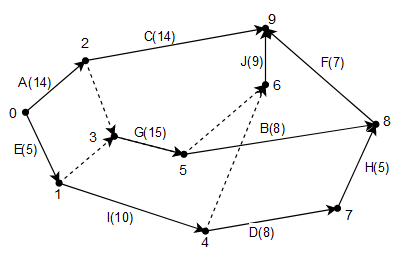
\includegraphics[width=0.7\linewidth]{./img/graf-2.PNG}
              \caption{Porządek wykonywania zadań w postaci grafu krawędziowego.}
              \label{fig:graf-2}
          \end{figure}
          Rysunek ~\ref{fig:graf-2} przedstawia porządek wykonywania zadań w postaci grafu krawędziowego wraz z posortowanymi wierzchołkami.
    \item Obliczam najwcześniejsze momenty rozpoczęcia:
          \begin{flalign*}
               & T_p0 = 0                                                        &  & \\
               & T_p1 = 0 + 5 = 5                                                &  & \\
               & T_p2 = 0 + 14 = 14                                              &  & \\
               & T_p3 = \max{(5 + 0, 14 + 0)} = 14                               &  & \\
               & T_p4 = 5 + 10 = 15                                              &  & \\
               & T_p5 = 14 + 15 = 29                                             &  & \\
               & T_p6 = \max{(15 + 0, 29 + 0)}= 29                               &  & \\
               & T_p7 = 15 + 8 = 23                                              &  & \\
               & T_p8 = \max{(29 + 8, 23 + 5)} = \max{(37, 28)} = 37             &  & \\
               & T_p9 = \max{(5 + 14, 29 + 9, 37 + 7)} = \max{(17, 38, 44)} = 44 &  & \\
          \end{flalign*}
    \item Obliczam najpóźniejszy moment zakończenia zadania:
          \begin{flalign*}
               & T_k9 = 44                                            &  & \\
               & T_k8 = 44 - 7 = 37                                   &  & \\
               & T_k7 = 37 - 5 = 32                                   &  & \\
               & T_k6 = 44 - 9 =  35                                  &  & \\
               & T_k5 = \min{(35 - 0, 37 - 8)} = \min{(35, 29)} = 29  &  & \\
               & T_k4 = \min{(35 - 0, 32 - 8)} = \min{(35, 24)} = 24  &  & \\
               & T_k3 = 29 - 15 = 14                                  &  & \\
               & T_k2 = \min{(44 - 14, 14 - 0)} = \min{(30, 14)} = 14 &  & \\
               & T_k1 = \min{(14 - 0, 24 - 10)} = \min{(14, 14)} = 14 &  & \\
               & T_k0 = \min{(14 - 14, 14 - 5)} = \min{(0, 9)} = 0    &  & \\
          \end{flalign*}
    \item Powyższe obliczenia nanoszę na graf, a następnie określam ścieżkę krytyczną
          poprzez połączenie wszystkich węzłów, gdzie najwcześniejszy moment rozpoczęcia (\(T_p\)) jest identyczny z najpóźniejszym
          momentem zakończenia zadania (\( T_k\)).
          \begin{figure}[H]
              \centering
              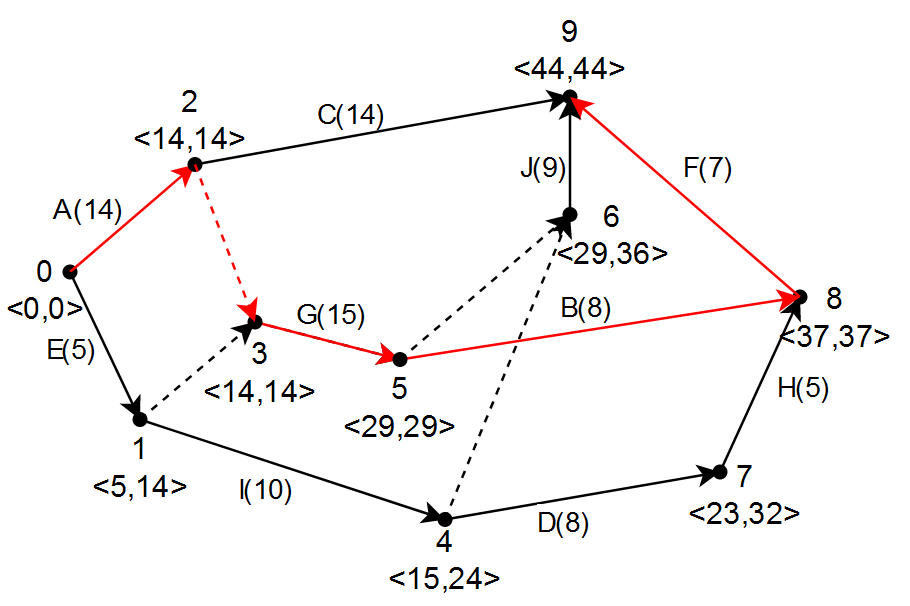
\includegraphics[width=0.7\linewidth]{./img/graf-3.PNG}
              \caption{Wyznaczona ścieżka krytyczna.}
              \label{fig:graf-3}
          \end{figure}
          Wyznaczona ścieżka krytyczna została zaznaczona na rysunku ~\ref{fig:graf-3} czerwonym kolorem.
\end{enumerate}
Czas potrzebny na przebycie ścieżki krytycznej to 44 jednostki czasu.
\subsection{Harmonogram o minimalnym czasie wykonania}
W celu uzyskania minimalnego czasu wykonania całego przedsięwzięcia zadanie programowania liniowego
zostało zapisane w języku modelowania AMPL.
\lstinputlisting[caption=Model w języku AMPL]{./src/model-1.mod}
\lstinputlisting[caption=Dane w języku AMPL]{./src/dane-1.dat}
\begin{lstlisting}[caption=Rozwiązanie znalezione solwerem minos]
    MINOS 5.51: optimal solution found.
    5 iterations, objective 44
    == 1 ==========================
\end{lstlisting}
Rozwiązanie zadania liniowego solwerem MINOS również znajduje wartość 44 jednostek czasu jako minimalny czas realizacji.
% To do: wstawić harmonogram
\subsection{Minimalny czas realizacji przedsięwzięcia przy określonym budżecie}
W ogólnym przypadku dobieramy zadania do skrócenia sprawdzając czy ich skrócenie jest możliwe.
Aby to zrobić należy odjąć od czasu trwania zadania jego czas minimalny.
W ten sposób uzyskujemy liczbę jednostek czasu, o które możemy skrócić zadanie.
W momencie kiedy mamy już zadania, które moglibyśmy potencjalnie skrócić należy wybrać
ścieżki do skrócenia o najniższym koszcie.
\begin{table}[H]
    \centering
    \begin{tabular} {| c | c | c | c | c | c |}
        \hline
        Zadanie & \(t\) & Poprzedniki & \(\alpha\) & \(t^{min}\) & \(t^{dif}\) \\
        \hline
        A       & 14    &             & 70         & 8           & 6           \\
        \hline
        B       & 8     & G           & 5          & 3           & 5           \\
        \hline
        C       & 14    & A           & 1          & 1           & 13          \\
        \hline
        D       & 8     & I           & 50         & 3           & 5           \\
        \hline
        E       & 5     &             & 90         & 5           & 0           \\
        \hline
        F       & 7     & B,H         & 80         & 3           & 4           \\
        \hline
        G       & 15    & A,E         & 75         & 6           & 9           \\
        \hline
        H       & 5     & D           & 100        & 1           & 4           \\
        \hline
        I       & 10    & E           & 50         & 6           & 4           \\
        \hline
        J       & 9     & G,I         & 20         & 5           & 4           \\
        \hline
    \end{tabular}
    \caption{Uzupełnione dane projektu o \(t^{dif}\).}
    \label{tab:dane_uzup}
\end{table}
Ze względu na modyfikację zadania należy wprowadzić dodatkowe zmienne do modelu matematycznego: \\
\(td_j\) - możliwy czas do skrócenia zadania \(j\) \\
\(tr_j\) - czas o jaki skracamy zadanie \(j\) \\
\(c_j\) - koszt skrócenia aktywności \(j\). \\ \\
Defniujemy również dodatkowe ograniczenia:
\begin{align*}
    \sum c_{ij} \cdot tr_{ij} \leq 200 \forall (i, j) \in R \\
    T_j \geq T_i + p_{ij} - tr_{ij} \forall (i,j) \in R \\
    0 \leq tr_{ij} \leq td_{ij}
\end{align*}
Modyfikujemy również funkcję celu: 
\begin{align*}
    min T_9
\end{align*}
\lstinputlisting[caption=Model w języku AMPL]{./src/model-2.mod}
\lstinputlisting[caption=Dane w języku AMPL]{./src/dane-2.dat}
\subsection{Dobór zadań przy wprowadzonym ograniczeniu NS}
\subsection{Najkrótszy czas wykonania przedsięwzięcia, gdy zadanie B nie może zakończyć się przed zakońćzeniem zadania A}
\newpage
\lstlistoflistings
\listoffigures
\listoftables

\end{document}
